\documentclass[11pt]{article}
\usepackage[utf8]{inputenc}
\usepackage[T1]{fontenc}
\usepackage{graphicx}

\usepackage[usenames,dvipsnames,svgnames,table]{xcolor}

\usepackage{subfigure}
\usepackage{xcolor}
\usepackage{hyperref}
\include{defs}

\usepackage{lipsum}
%\usepackage[spanish]{babel}

\usepackage{booktabs}
\usepackage{array}
\usepackage{tabularx,multirow}

%\setcounter{page}{0}

%%%%%%%%%%%%%%%
% Title Page
\title{}
\author{}
\date{}
%%%%%%%%%%%%%%%

\begin{document}
\maketitle

%\tableofcontents
\clearpage
\clearpage
\section*{Welcome!}
Welcome to the beautiful city of Braga! We are very happy that you all have joined us for this LTTA (learning, teaching and training activities), where we are going to talk and learn about Artificial Intelligence, all within the scope of the FAIaS project. 

This LTTA will be quite informal, but it will serve as a networking point to meet people from very different places (such as Portugal, Spain or Belgium), we will have some good food together and last but not least we will have lots of fun. 

FAIaS fosters the knowledge and skills around Artificial Intelligence and Machine Learning at European schools, funded under an Erasmus+ KA201 innovation in schools project. The project will run until August 2023.

The goals of FAIaS are: 
\begin{enumerate}
    \item To foster the knowledge and skills around Artificial Intelligence and Machine Learning in European schools.
    \item To achieve goal \#1 in a way that is as inclusive as possible, with special attention to gender, economically and socially disadvantaged students, among others. 
    \item To raise awareness of the technical, social and ethical implications of Artificial Intelligence and Machine Learning.
\end{enumerate}

Its expected outcomes are:
\begin{enumerate}
    \item High-quality, open learning materials and experiences for educators and learners on AI and ML.
    \item Easy-to-use web-based (open source) software tools to support learning of AI and ML.
    \item Organization of activities for educators and learners on AI and ML (and make our learning materials, experiences and tools known).
\end{enumerate}


\subsection*{About the LTTA}

During the short-term training activity (4 days) organized in Braga during the next days, the 20 FAIAS educators selected by the partners from the participating countries (9 from Belgium, 6 from Spain and 5 from Portugal) will meet the FAIaS partners and not only will be fully trained on the FAIaS objectives and introduced to the FAIAS outputs, but, most of all, they will be officially designated and invested with their role within the FAIaS project and become a FAIaS Ambassador.

To be FAIaS Ambassador means to be ready, eager and willing to collaborate, contribute, and be committed to the FAIaS project implementation. FAIaS Ambassadors will be a core figure within the project and the role will consist of and will require to:
\begin{itemize}
    \item Contribute in the drafting and revision of the main project outputs (collecting also contributions and suggestions from the local teachers)
    \item Act as a liaison between the FAIaS partners and the FAIaS local teachers communities 
    \item Train and support the local school teachers and colleagues to actively take part to FAIAS activities
    \item Encourage teachers to collaborate, to share ideas and projects, to use the FAIAS repository and tools 
    \item Moderate the FAIaS local community 
    \item Support with the dissemination of the FAIaS results to the school communities
\end{itemize}

During the short-term training activity the FAIaS ambassadors will not only be “theoretically” trained on the FAIAS results. Interactive and collaborative sessions will be organized in order to share experience and proposals between the FAIaS Ambassadors and foster a strong collaboration among them.

\subsection*{Important Places}

\begin{enumerate}
    \item Meeting place: 
gnration.
Praça Conde de Agrolongo 

\item Breakfast:
Doce Carmo.
R. do Carmo

\item Lunches:
Mostarda e Chocolate.
Praça Conde de Agrolongo

\item Dinners (Tuesday and Thursday):
Atravessado.
R. de Santo António das Travessas 30

\item Banquet (Wednesday):
Bem-me-quer.
Campo das Hortas, 6
\end{enumerate}

\begin{figure}[ht]
    \centering
    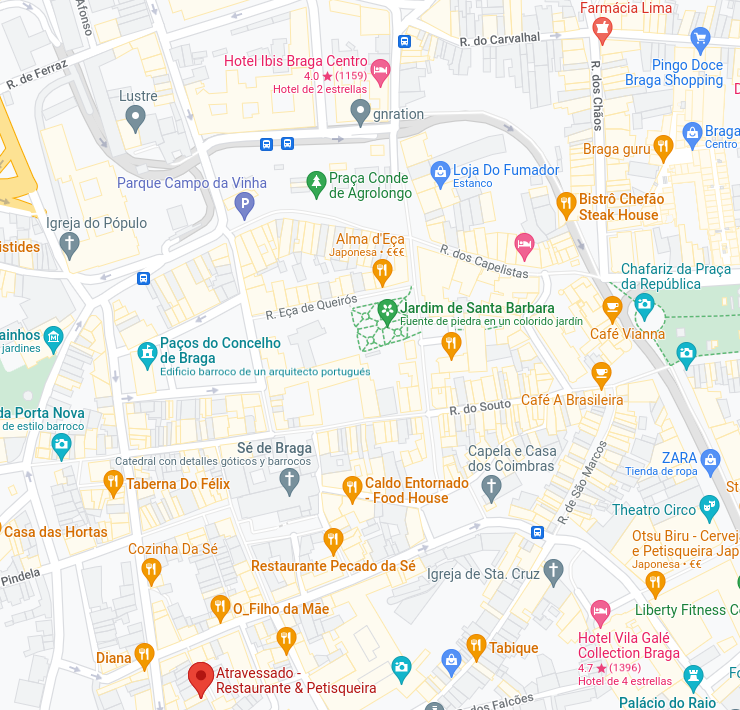
\includegraphics[scale=0.45, keepaspectratio]{braga_map.png}
    \caption{Braga map}
    \label{figure:map}
 \end{figure}

\begin{table}
    \renewcommand{\arraystretch}{1.4}
     \begin{center}
     %\rowcolors{2}{gray!15}{white}
      \begin{tabular}{m{6cm} m{8cm}} % 2 cols 
        \hline
        \rowcolor{gray!35}\centering\arraybackslash\textbf{Day} & \centering\arraybackslash\textbf{Activity} \\
        \hline%\hline
        
        %\rowcolor{white}\multirow[t]{-2}{*}{\textbf{Tuesday, May 31 2022}} & \textbf{16:00 Welcome}(and activity)
        \centering\textbf{Tuesday, May 31 2022} &  \textbf{16:00 Welcome} (and activity) \newline
        \textbf{17:30 Talks by participants} \newline
        - ``Machine Learning in Education'' by Pablo Dúo Terrón \newline
        - ``Overview of AI activities developed by la Scientothèque'' by Yann-Aël Le Borgne \newline
        - ``The use of filters in a deep neural network for image recognition'' by Natacha Gesquière
        \newline
        \textbf{19:00 End} \newline
        \textbf{20:00 Dinner}
        \\ %\hline
        %\cdashline{2-3}
        \rowcolor{gray!15}
        \centering\textbf{Wednesday, June 1 2022} & \textbf{09:30 Breakfast} \newline \textbf{10:00 Intro to AI} \newline \textbf{13:00 Lunch} \newline 
        \textbf{15:00 Talks by participants II} \newline
        - ``AI Generation'' by Maria Inmaculada Caruana\newline
        - ``XR in education'' by Peter De Deyn \newline
        - ``Problem solving with Machine Learning and Scratch'' by Álvaro Molina
        \newline
        \textbf{16:15 LearningML} \newline
        \textbf{17:30 Guided visit through Braga} \newline
        \textbf{19:00 End} \newline
        \textbf{20:00 Banket}
        \\ 
        \centering\textbf{Thursday, June 2 2022} & \textbf{09:30 Breakfast} \newline \textbf{10:00 Example lessons} % Machine Learning in Citizenship lessons by Liliana Carrillo 
        \newline \textbf{13:00 Lunch} \newline
        \textbf{15:00 Preparation:} Create your lesson
        \newline
        \textbf{17:00 Presentations} \newline
        \textbf{17:30 End} \newline
        \textbf{20:00 Dinner} \\
        \rowcolor{gray!15}
        \centering\textbf{Friday, June 3 2022} &
        \textbf{09:30 Breakfast} \newline 
        \textbf{10:00 Presentation time} \newline 
        \textbf{12:00 Reflection and discussion time} \newline 
        \textbf{13:00 Lunch and farewell} \\
        \bottomrule%\hline
    \end{tabular}
      \caption[LTTA program]{LTTA program.}
      \label{tab:program}
     \end{center}
    \end{table}

    \newpage

\section*{Participants}
\noindent
\begin{minipage}{0.3\textwidth}
\centering
\includegraphics[width=5cm]{images/img1.jpeg}
\end{minipage}
\hfill
\begin{minipage}{0.6\textwidth}\raggedright
\color{color1}\uppercase{\textbf{Marjon Blondeel}}
\color{color2}\hspace{0.2cm}\includegraphics{flags/be.png}
\\
software/AI developer at VUB\\
{\footnotesize Researcher in AI until 2015. Now focused on developing AI applications and giving trainings on AI. During 1 year I also worked as a teacher in secondary school and I have many years of experience as a teaching assistant and lecturer in higher education. I've taught basic courses for informatics students, but also programming courses for other students such as Bio-Engineering students. }\\
\end{minipage}
\newline\newline\newline

\noindent
\begin{minipage}{0.3\textwidth}
\centering
\includegraphics[height=5cm]{images/img0.jpg}
\end{minipage}
\hfill
\begin{minipage}{0.6\textwidth}\raggedright
\color{color1}\uppercase{\textbf{Macu Caruana}}
\color{color2}\hspace{0.2cm}\includegraphics{flags/es.png}
\hspace{0.2cm}\textit{@macucaruana}
\\
Primary Teacher at Teacher\\
{\footnotesize Keen on Technology and education. I love sports, fan of Rafa Nadal. I also like photography and living as close as possible to the sea.}\\
\end{minipage}
\newline\newline\newline

\noindent
\begin{minipage}{0.3\textwidth}
\centering
\includegraphics[height=5cm]{images/img3.png}
\end{minipage}
\hfill
\begin{minipage}{0.6\textwidth}\raggedright
\color{color1}\uppercase{\textbf{Meritxell Díaz Coque}}
\color{color2}\hspace{0.2cm}\includegraphics{flags/es.png}
\\
Researcher at King Juan Carlos University\\
{\footnotesize I am a Electrical Engineer in Telecommunications and in Aerospace Engineer, currently working as a researcher in the FAIaS project. In this project, we are trying to teach Artificial Intelligence in high schools. I'm passionate about programming and artificial intelligence.}\\
\end{minipage}
\newline\newline\newline

\noindent
\begin{minipage}{0.3\textwidth}
\centering
\includegraphics[height=5cm]{images/img0.jpg}
\end{minipage}
\hfill
\begin{minipage}{0.6\textwidth}\raggedright
\color{color1}\uppercase{\textbf{Johan Loeckx}}
\color{color2}\hspace{0.2cm}\includegraphics{flags/be.png}
\hspace{0.2cm}\textit{@aibrussels}
\\
Researcher at Artificial Intelligence Lab Brussels (VUB)\\
{\footnotesize I have three passions: music, education \& AI.  have founded a Freinet school in Brussels, I have done research on using AI to educate people on music, and am currently mainly involved with lifelong learning of AI.}\\
\end{minipage}
\newline\newline\newline

\noindent
\begin{minipage}{0.3\textwidth}
\centering
\includegraphics[height=5cm]{images/img5.jpeg}
\end{minipage}
\hfill
\begin{minipage}{0.6\textwidth}\raggedright
\color{color1}\uppercase{\textbf{Gregorio Robles}}
\color{color2}\hspace{0.2cm}\includegraphics{flags/es.png}
\hspace{0.2cm}\textit{@gregoriorobles}
\\
Full Professor at Universidad Rey Juan Carlos\\
{\footnotesize I am a Full Professor at the Universidad Rey Juan Carlos, a public university in the South of Madrid.}\\
\includegraphics[height=0.35cm]{figs/internet.png}\hspace{0.1cm}{\footnotesize \color{color1}\url{https://gsyc.urjc.es/~grex/}}
\end{minipage}
\newline\newline\newline

\noindent
\begin{minipage}{0.3\textwidth}
\centering
\includegraphics[width=5cm]{images/img6.png}
\end{minipage}
\hfill
\begin{minipage}{0.6\textwidth}\raggedright
\color{color1}\uppercase{\textbf{Pablo Duo Terron}}
\color{color2}\hspace{0.2cm}\includegraphics{flags/es.png}
\hspace{0.2cm}\textit{@esparaTIC}
\\
Director and teacher  in Primary School at ministry of education and vocational training\\
{\footnotesize Doctoral student in education 
Master TIC and Educational Inspection 
Degree in primary school and physical education  
2nd best teacher of Primary School in Spain 2021
Coordinator and tutor of the Future Classroom courses of the (national institute of technology teacher training in Spain) INTEF
Tutor of the Computational Thinking and Artificial Intelligence school of the INTEF
STEM Diagnostic Test Coordinator INEE}\\
\includegraphics[height=0.35cm]{figs/internet.png}\hspace{0.1cm}{\footnotesize \color{color1}\url{educaciontic.es}}
\end{minipage}
\newline\newline\newline



\newpage
\section*{Notes}

\end{document}
